%    Documentation for PRU ADC Project
%    Copyright (C) 2016  Gregory Raven
%
%    This program is free software: you can redistribute it and/or modify
%    it under the terms of the GNU General Public License as published by
%    the Free Software Foundation, either version 3 of the License, or
%    (at your option) any later version.
%
%    This program is distributed in the hope that it will be useful,
%    but WITHOUT ANY WARRANTY; without even the implied warranty of
%    MERCHANTABILITY or FITNESS FOR A PARTICULAR PURPOSE.  See the
%    GNU General Public License for more details.
%
%    You should have received a copy of the GNU General Public License
%    along with this program.  If not, see <http://www.gnu.org/licenses/>.

\chapter{Prototype Cape Detail}




The proto-cape schematic is simple, and is composed of a single component, the MCP3008 ADC.

\begin{figure}[H]
	\centering
	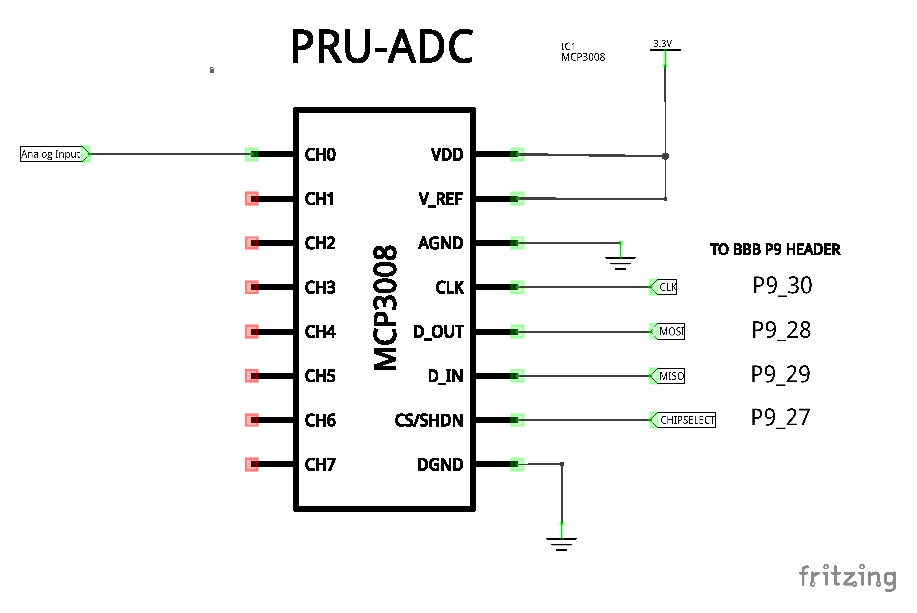
\includegraphics{../../pcb/pru_adc_schematic_schem}
	\centering\bfseries
	\caption{PRU-ADC Cape Breadboard}
\end{figure}

The ``Cape'' was built on an Adafruit proto-cape:

\url{https://www.adafruit.com/products/572}

Here is a breadboard diagram from Fritzing which shows how the proto-cape
is wired:

\begin{figure}[H]
	\centering
	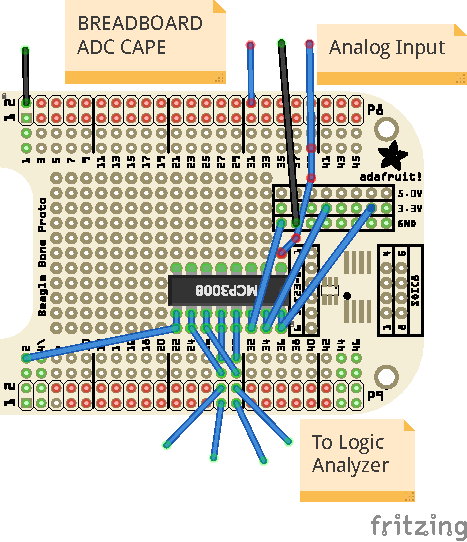
\includegraphics[]{../../pcb/adafruit_proto_cape_bb-crop}
	\centering\bfseries
	\caption{PRU-ADC Cape Breadboard}
\end{figure}

In addition to the header pins required to plug into the BBB, extra rows of headers were soldered to the top of the breadboard.  This allows easy connection to the Discovery Analog 2 as seen in the following photograph.

\begin{figure}[H]
	\centering
	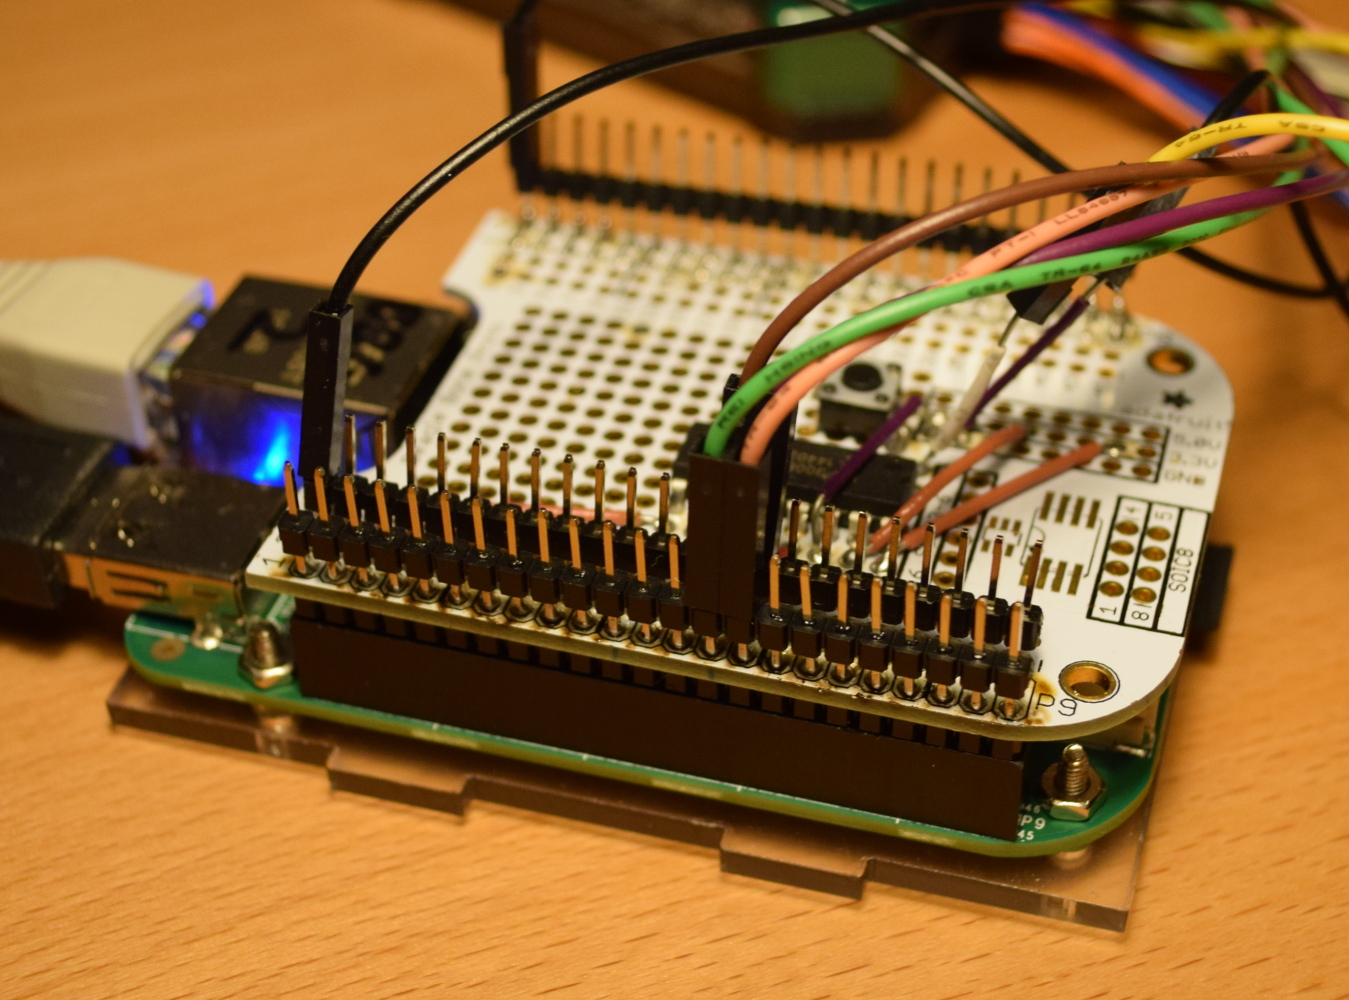
\includegraphics{photos/DSC_0025}
	\centering\bfseries
	\caption{PRU-ADC Cape Breadboard}
\end{figure}

